\documentclass[ejs]{imsart}

%\pdfoutput=1

\RequirePackage{mathrsfs,mathtools,latexsym,enumerate,amsmath, amsthm, amssymb,hyperref,amsfonts,framed,tikz,enumerate,bbm,appendix,soul}
% \RequirePackage{pdftricks} % throws warnings if used
\RequirePackage{romanbar}
\RequirePackage{MnSymbol} 
\RequirePackage{multirow,mathtools,latexsym, mathrsfs,framed,listings,mleftright,enumitem}
\RequirePackage[colorlinks,citecolor=blue,urlcolor=blue]{hyperref}
\RequirePackage{graphicx}
\RequirePackage{sourcecodepro}
\RequirePackage{xcolor}
\RequirePackage{dsfont}
\RequirePackage{parskip}
\RequirePackage{tikz}
\usetikzlibrary{positioning}
%\arxiv{2310.07399}

\startlocaldefs
\theoremstyle{plain}% default
\newtheorem{prototheorem}{Theorem}

\newtheorem{theorem}[prototheorem]{Theorem}
\newtheorem{lemma}[prototheorem]{Lemma}
\newtheorem{proposition}[prototheorem]{Proposition}
\newtheorem{corollary}[prototheorem]{Corollary}
%\newtheorem{definition}[prototheorem]{Definition}
%\newtheorem{remark}[prototheorem]{Remark}
\newtheorem{example}[prototheorem]{Example}

\theoremstyle{remark}
\newtheorem{definition}{Definition}
\newtheorem{remark}{Remark}
\newtheorem{assumption}{Assumption}

\DeclarePairedDelimiter\ceil{\lceil}{\rceil}
\DeclarePairedDelimiter\floor{\lfloor}{\rfloor}
\DeclarePairedDelimiter\set{\{}{\}}
\newcommand{\norm}[1]{\left\lVert#1\right\rVert}
\newcommand{\R}{\mathbb{R}}
\newcommand{\prb}{\mathbb{P}}
\newcommand{\ev}[1]{\mathbb{E} \left[ #1 \right]}
\newcommand{\evsub}[2]{\mathbb{E}_{#1} \left[ #2 \right]}
\newcommand{\var}[1]{\text{Var} \left( #1 \right)}
\newcommand{\sigf}{\mathcal{F}}
\DeclarePairedDelimiter{\abs}{\lvert}{\rvert}
\newcommand{\dd}{\, \text{d}}
\newcommand{\eps}{\varepsilon}
\newcommand{\differential}{D}
\newcommand{\mnorm}[1]{\left\| #1 \right\|} %matrix norm
\newcommand{\Z}{\ensuremath \mathbb{Z}}
\newcommand{\W}{\boldsymbol{\mathcal{W}}}
\newcommand{\PM}{\ensuremath \mathcal{P}}
\newcommand{\J}{\mathrm{Couplings}}
\newcommand{\law}{\operatorname{Law}}
\newcommand{\opnorm}[1]{\left\| #1 \right\|_{\mathsf{op}}} 
\newcommand{\wnorm}[1]{\left\| #1 \right\|_{\mathsf{w}}} 
\newcommand{\wonenorm}[1]{\left\| #1 \right\|_{\mathsf{w},1}} 



  
\newcommand{\lb}[1]{{\lfloor #1 \rfloor_h}}
\newcommand{\ub}[1]{{\lceil #1 \rceil_h}}
\newcommand{\rn}[1]{\Romanbar{#1}}

\makeatletter
\let\c@author\relax
\makeatother

\usepackage[backend=biber,backref=true,style=numeric,giveninits=true,maxbibnames=9]{biblatex}
\addbibresource{nawaf.bib}
\endlocaldefs
\DeclareHookRule{begindocument}{imsart}{after}{biblatex}

\begin{document}


\begin{frontmatter}
\title{Self-Tuning Hamiltonian Monte Carlo: Adaptively Sampling Path Lengths} 
\runtitle{Self-Tuning HMC}


\begin{abstract} We present a novel framework for tuning Hamiltonian Monte Carlo and an application to dynamically setting integration time using a U-turn condition similar to that employed by the widely used no-U-turn sampler.
\end{abstract}


\begin{aug}
\author[A]{\fnms{Nawaf} \snm{Bou-Rabee}\ead[label=e1]{nawaf.bourabee@rutgers.edu}\orcid{0000-0001-9280-9808}},
\author[B]{\fnms{Bob} \snm{Carpenter}\ead[label=e2]{bcarpenter@flatironinstitute.org}\orcid{}}, 
\and
\author[C]{\fnms{Milo} \snm{Marsden}\ead[label=e3]{mmarsden@stanford.edu}\orcid{}}
\address[A]{Department of Mathematical Sciences, Rutgers University Camden,  \\  \printead[presep={}]{e1}}
\address[B]{Center for Computational Mathematics, Flatiron Institute,  \\ \printead[presep={}]{e2}}
\address[C]{Department of Mathematics, Stanford University,  \\ \printead[presep={}]{e3}}
\runauthor{N. Bou-Rabee, B. Carpenter, M. Marsden}
\end{aug}



\begin{keyword}[class=MSC]
\kwd[Primary ]{60J22} % Computational methods in Markov chains
\kwd[; Secondary ]{65C05} % Monte Carlo methods
\kwd{65P10} % Numerical methods for Hamiltonian systems including symplectic integrators
\kwd{60J05} % Discrete-time Markov processes on general state spaces
\kwd{62F15} % Bayesian inference
\end{keyword}


\begin{keyword}
\kwd{Markov chain Monte Carlo}
\kwd{Hamiltonian Monte Carlo}
\kwd{Self-Tuning}
\kwd{High Dimensions}
\end{keyword}
\end{frontmatter}


\section{Introduction}

\subsection{Motivation}

Tuning the parameters of Markov chain Monte Carlo (MCMC) algorithms is critical to their  performance, but notoriously difficult in practice.  The challenge of tuning is particularly acute for Hamiltonian Monte Carlo (HMC), where the tuning of path length \cite{HoGe2014,BoSa2017,betancourt2017conceptual,kleppe2022connecting}, step length \cite{BePiRoSaSt2013,betancourt2014optimizing,biron2023automala}, and pre-conditioner \cite{GiCa2011,kleppe2016adaptive,whalley2024randomized}~frequently presents a complex trade off between computational cost and mixing.   The successful self-tuning of path length provided by the no-U-turn sampler (NUTS) has led to its widespread adoption as the default sampler in probabilistic programming languages \cite{carpenter2016stan,salvatier2016probabilistic,nimble-article:2017,ge2018t,phan2019composable}.

In NUTS, the path length is  dynamically set according to a no-U-turn termination criteria, which roughly speaking stops the underlying Hamiltonian trajectory whenever it doubles back \cite{HoGe2014,betancourt2017conceptual}. The main idea is to numerically integrate the Hamiltonian equations forward/backward in time until a no-U-turn criterion is met. A point along this discrete path is randomly selected such that: (i) the resulting sampler has the correct distribution; and (ii) points far from the starting point are more likely to be selected.  While the original NUTS algorithm used a slice sampler, the latest version is based on a multinomial procedure \cite[Appendix A]{betancourt2017conceptual}.  The correctness and basic properties of NUTS has been the subject of several recent works \cite{andrieu2020general, durmus2023convergence}.   

Can other parameters such as the step length and pre-conditioner be similarly self-tuned?   
This paper addresses this question by presenting a novel framework for adaptively setting HMC parameters such as the path length, step length, and pre-conditioner.  

\begin{figure}
\begin{flushleft}
$\textrm{GeneralSelfTuneHmcStep}(\theta)$
\vspace*{2pt}
\hrule
\vspace*{2pt}
\begin{tabular}{ll}
$\theta \in \mathbb{R}^d$: & position
\\
$\rho \in \mathbb{R}^d$: & momentum
\\
$\alpha \in \mathcal{A}$: & tuning parameter
\end{tabular}
\vspace*{4pt}
\hrule
\vspace*{8pt}
Set $\theta_0 = \theta$.
\\[4pt]
Resample momentum $\rho_0 \sim \textrm{Normal}(0, \textrm{I}_{d \times d}).$
\\[4pt]
Sample tuning parameter $\alpha \sim p(\cdot \mid \theta_0, \rho_0)$.
\\[4pt]
Set proposal $(\theta^*, \rho^*) = F(\alpha)(\theta_0, \rho_0)$.
\\[4pt]
Sample $\mathcal{U} \sim \textrm{Uniform}(0, 1)$.
\\[4pt]
Return $\theta^*$ 
if $\mathcal{U} < e^{-\Delta H(\theta_0,\rho_0)} \, \dfrac{p\left(\alpha \, | \, \mathcal{S} \circ F(\alpha)(\theta_0, \rho_0) \right)}{p \left(\alpha\, | \, \theta_0, \rho_0 \right)} $
else return $\theta_0$.
\vspace*{4pt}
\hrule
\caption{\it {\bfseries General self-tuning HMC step}.  This algorithm differs from standard HMC in the sampling of the tuning parameters and subsequent adjustment of acceptance proability.  Here we used the shorthand $\Delta H(\theta, \rho) := H \circ F(\alpha)(\theta,\rho) - H(\theta, \rho)$ and $I_{d \times d}$ denotes the $d \times d$ identity matrix.}
\label{fig:general-self-tuning-step}
\end{flushleft}
\end{figure}

\subsection{General framework for adaptively setting HMC parameters}

Hamiltonian Monte Carlo (HMC) is a class of MCMC methods for sampling distributions of the form \begin{equation} \label{eq:target}
\mu(d\theta, d\rho) \propto e^{-H(\theta,\rho)} m( d\theta \, d\rho) \;, 
\end{equation}
which have a density relative to Lebesgue measure $m$ on phase space $\mathbb{R}^{2d}$.  We assume for simplicity the case of a separable Hamiltonian with unit metric, i.e. \[
H(\theta,\rho) = U(\theta) + \frac{1}{2} \left|\rho\right|^2 \;, 
\]
for a continuously differentiable function $U: \mathbb{R}^d \to \mathbb{R}$ such that $\int e^{-U} d\theta < \infty$. 

A defining ingredient of any HMC algorithm is a reversible, volume-preserving map $F(\alpha): \mathbb{R}^{2d} \to \mathbb{R}^{2d}$ where $\alpha$ is a tuning parameter \cite{BoSaActaN2018}.  Note that $\mathcal{S} \circ F(\alpha)$ is a volume-preserving involution where $\mathcal{S}(\theta, \rho) = (\theta, -\rho)$ \cite{ChBaCa2023}.  We suppose that the tuning parameter $\alpha$
takes values in a set $\mathcal{A}$ where $(\mathcal{A}, \mathcal{B}, \eta)$ is a measure space with Borel $\sigma$-algebra $\mathcal{B}$ and background measure $\eta$.

To self-tune the parameter $\alpha$, the state space $\mathbb{R}^{2d}$ is enlarged to a product space $\mathbb{R}^{2d} \times \mathcal{A}$. On this enlarged space, an enlarged target measure is defined by specifying a conditional density of $\alpha$ given $(\theta, \rho)$ \begin{equation} \label{eq:enlarged_target}
\mu_e(d\theta, d\rho, d\alpha) \propto  e^{-H(\theta, \rho)} \, p( \alpha \, | \, \theta, \rho) \, (m \otimes \eta) (d\theta \, d\rho  \, d\alpha) \;.
\end{equation}  Note that the $(\theta, \rho)$-marginal of $\mu_e$ is the desired target measure $\mu$.

Figure~\ref{fig:general-self-tuning-step} describes a transition step of the general self-tuning HMC algorithm. This transition step leaves invariant $\mu_e$.  Indeed, it is a Gibbs sampler aimed at $\mu_e$.  The accept/reject step is a Metropolis step on the enlarged space with acceptance probability \begin{equation} \label{eq:acceptanceprobability}
a_e(\theta_0, \rho_0, \alpha) = 1 \wedge \left(  e^{-\Delta H(\theta_0,\rho_0)} \, \dfrac{p\left(\alpha \, | \, \mathcal{S} \circ F(\alpha)(\theta_0, \rho_0) \right)}{ p \left(\alpha\, | \, \theta_0, \rho_0 \right)} \right) \;.
\end{equation} This accept/reject step is correct/valid since the proposal move on the enlarged space $(\theta_0, \rho_0, \alpha) \mapsto (\theta^*, \rho^*, \alpha)$ is reversible  and leaves invariant $m \otimes \eta$.  A self-contained proof of correctness is provided in Appendix~\ref{app:proof_of_correctness}.


Additionally, one can use this framework to randomize the time integrator for the Hamiltonian flow, as in \cite{BouRabeeMarsden2022,BouRabeeKleppe2023}.  In this case, the tuning parameter would specify a particular time integrator within a parametric family of time integrators that are individually reversible and volume-preserving.  In certain representative models, randomized time integrators can have a provably better complexity for Hamiltonian McMC than the standard leapfrog integrator \cite{shen2019randomized,ErgodicityRMMHYB,Cao_2021_IBC,BouRabeeMarsden2022,BouRabeeSchuh2023B,BouRabeeOberdoerster2023}.  


\subsection{Adaptively setting path lengths}

To both make this framework more concrete and  demonstrate its breadth, we now discuss a few examples of HMC samplers that adaptively set path lengths that fit within this framework.  

\begin{example}[Randomized HMC]
Consider $F(\alpha)(\theta, \rho) = \varphi_\alpha(\theta, \rho)$ where we have introduced the the exact Hamiltonian flow $\varphi_{\alpha}: \mathbb{R}^{2d} \to \mathbb{R}^{2d}$ at time $\alpha \ge 0$. Take $(\mathcal{A},\eta) = ([0, \infty), m)$ and $p(\alpha \mid \theta, \rho) = \lambda e^{- \lambda \alpha}$ where $\lambda > 0$. In this case, $\alpha$ is selected from an exponential distribution with parameter $\lambda$, the proposal move is always accepted, and Figure~\ref{fig:general-self-tuning-step} essentially describes a draw from randomized HMC at the first jump time \cite{BoSa2017,BoEb2022}.
\end{example}

\begin{example}[Adapting Path Lengths in Exact HMC]
Consider once again $F(\alpha) = \varphi_\alpha(\theta, \rho)$ where  $\varphi_{\alpha}: \mathbb{R}^{2d} \to \mathbb{R}^{2d}$ is the exact Hamiltonian flow map at time $\alpha \ge 0$ and let $(\mathcal{A}, \eta) = ([0, \infty), m)$. Let $\tau(\theta, \rho):\mathbb{R}^{2d} \to (0, \infty)$ be any measurable function.  Take \[ p(\alpha \mid \theta, \rho) \, = \,  \dfrac{1}{\tau(\theta, \rho)} \mathds{1}_{[0,\tau(\theta, \rho)]}( \alpha ) \;.
\] In this case, we select $\alpha$ uniformly at random from  $[0,\tau(\theta, \rho)]$. 
As a shorthand, let $\tau_1 = \tau(\theta_0, \rho_0)$ and $\tau_2 = \tau(\mathcal{S} \circ \varphi_{\alpha}(\theta_0, \rho_0))$.
Having selected $\alpha$ from this distribution, the acceptance probability in \eqref{eq:acceptanceprobability} reduces to \[ a_e(\theta_0, \rho_0, \alpha) \, = \, 1 \wedge \left( \frac{\tau_1}{\tau_2} \mathds{1}_{ \{  \tau_2 \geq \alpha \} } \right) \;, \] since $\Delta H(\theta_0, \rho_0) = 0$ for the exact Hamiltonian flow.  The indicator in this Metropolis ratio indicates that  $p(\alpha \mid \mathcal{S} \circ \varphi_{\alpha}(\theta_0, \rho_0)) \ne 0$.


Conditions avoiding $U$-turns in the exact Hamiltonian flow can be used to define $\tau(\theta, \rho)$.  There are several ways to characterize such $U$-turn conditions. For example, here is a condition based on when the angle between the initial velocity $\rho_0 \in \mathbb{R}^d$ and the velocity $\rho_t \in \mathbb{R}^d$ at time $t \ge 0$ first exceeds $\pi/2$ \begin{equation} \label{eq:ct_angle}
\tau(\theta_0, \rho_0) \ := \ \inf\{ t > 0 ~:~ \rho_0 \cdot \rho_t \le 0 \} \;,
\end{equation} where we have introduced $(\theta_t, \rho_t) := \varphi_t(\theta_0, \rho_0)$ for $t \ge 0$.  Another condition is based on when the squared distance $\Gamma(t) := | \theta_0 - \theta_t|^2$ between the initial configuration $\theta_0 \in \mathbb{R}^d$ and the configuration $\theta_t \in \mathbb{R}^d$ at time $t \ge 0$ first decreases \begin{equation} \label{eq:ct_dist}
\tau(\theta_0, \rho_0) \ := \ \inf\{ t > 0 ~:~ \Gamma'(t) < 0 \} \;.
\end{equation}
These continuous-time $U$-turn conditions have discrete-time analogs, which are presented in Section~\ref{sec:uniform}.
\end{example}


\begin{example}[Adapting Path Lengths in Numerical HMC] \label{ex:numericalHMC}
Fix a step length $h>0$.  Let $\Phi_h: \mathbb{R}^{2d} \to \mathbb{R}^{2d}$ denote one step of the leapfrog integrator operated at step length $h$.  Consider $F(\alpha)(\theta, \rho) = \Phi_h^{\alpha}(\theta, \rho)$ where $\alpha$ is the \# of leap frog steps. Take $\mathcal{A} = \mathbb{N}$ and let $\eta$ be counting measure. Similarly to the above let $\tau: \mathbb{R}^{2d} \to \mathbb{N}$ be a measurable function and define \[ p(\alpha \mid \theta, \rho) = \frac{1}{\tau(\theta, \rho)} \mathds{1}_{\{0, \dots, \tau(\theta, \rho)-1\} }(\alpha) \;.  \]
Similarly to the above, the acceptance probability in \eqref{eq:acceptanceprobability} is \[
a_e(\theta_0, \rho_0, \alpha) \, = \, 
1 \wedge \left( e^{-\Delta H(\theta_0, \rho_0)} \frac{\tau_1}{\tau_2} \mathds{1}_{\{ \tau_2 \geq \alpha \} } \right) \;, \]
where we used the shorthand notation $\tau_1 = \tau(\theta_0, \rho_0)$ and $\tau_2 = \tau(\mathcal{S} \circ \Phi^{\alpha}_h(\theta_0, \rho_0))$.
\end{example}

The paper is organized as follows. Section~\ref{sec:uniform} expands on Example~\ref{ex:numericalHMC} by specifying the functions $\tau(\theta, \rho)$.   Section~\ref{sec:nonuniform} explains how to obtain robustness w.r.t.~step length by incorporating a mulitnomial procedure and biasing the selection of next states towards points further from the starting point.  



\section{Distributions over the number of steps} \label{sec:uniform}

To make the general notion of adaptive HMC concrete, we introduce a general sampler that adapts its number of steps each iteration and then evaluation several choices of distribution over the number of steps.  

\subsection{General step selection algorithm}

\newcommand{\pos}[2]{#1^{(#2)}}
\begin{figure}
\begin{flushleft}
$\textbf{TrajectoryTunedHmcStep}(\theta, \rho, \epsilon, \Sigma)$
\vspace*{2pt}
\hrule
\vspace*{2pt}
\begin{tabular}{ll}
$\theta \in \mathbb{R}^d$ & position
\\[2pt]
$\rho \in \mathbb{R}^d$ & momentum
\\[2pt]
$\epsilon \in (0, \infty)$ & step size
\\[2pt]
$\Sigma \in \mathbb{R}^{d \times d}$ & symmetric, positive definite metric
\end{tabular}
\vspace*{2pt}
\hrule
\vspace*{6pt}
$\pos{\theta}{0} = \theta$
\\[4pt]
$\pos{\rho}{0} \sim \textrm{normal}(0, \Sigma).$ \hfill (resample momentum)
\\[4pt]
$L \sim p(L \mid \pos{\theta}{0}, \pos{\rho}{0}, \epsilon, \Sigma)$ \hfill (Gibbs sample tuning parameters)
\\[4pt]
for $\ell$ from $0$ to $L - 1$ (inclusive):  \hfill ($L$ leapfrog steps)
\\[-4pt]
\null \qquad $\pos{\rho}{\ell + 1/2} = \pos{\rho}{\ell} - \frac{\epsilon}{2} \cdot \nabla \log p(\pos{\theta}{\ell})$ \hfill (half step momentum)
\\[-4pt]
\null \qquad $\pos{\theta}{\ell + 1} = \pos{\theta}{\ell} + \epsilon \cdot \Sigma^{-1} \cdot \pos{\rho}{\ell + 1/2}$ \hfill (full step position)
\\[-4pt]
\null \qquad $\pos{\rho}{\ell + 1} = \pos{\rho}{\ell + 1/2} - \frac{\epsilon}{2} \cdot \nabla \log p(\pos{\theta}{\ell + 1})$ \hfill (half step momentum)
\\[6pt]
$\theta^*, \rho^*, L^* = \pos{\theta}{L}, -\pos{\rho}{L}, L$  \hfill (proposal flips momentum)
\\[4pt]
$u \sim \textrm{uniform}(0, 1)$ \hfill (sample acceptance probability)
\\[4pt]
if
$u < \frac{\displaystyle p(\theta^*, \rho^*,  L^* \mid \epsilon, \Sigma)}
         {\displaystyle p(\pos{\theta}{0}, \pos{\rho}{0}, L^* \mid \epsilon, \Sigma)}$
\hfill (Metropolis adjust)
\\
\null \quad return $\left(\theta^*, \rho^*, L^* \right)$ \hfill (accept)
\\[4pt]
else
\\[-6pt]
\null \quad return $\null \quad \left( \pos{\theta}{0}, \pos{\rho}{0}, L^* \right)$ \hfill (reject)
\hrule
\caption{\it {\bfseries Self-tuning HMC step}.  This algorithm differs from HMC in sampling the tuning parameters each iteration and then adjusting the acceptance probability to ensure detailed balance.  The Gibbs proposal for the new number of steps $L$ is exact and always accepted.}
\label{fig:self-tuning-hmc}
\end{flushleft}
\end{figure}

Figure~\ref{fig:self-tuning-hmc} provides pseudocode for the general algorithm.  The joint density of the position, momentum and steps can be factored as
\begin{equation}
\frac{\displaystyle p\!\left(\theta^*, \rho^*,  L^* \mid \epsilon, \Sigma\right)}
         {\displaystyle p\!\left(\pos{\theta}{0}, \pos{\rho}{0}, L^* \mid \epsilon, \Sigma\right)}
\ = \ 
\frac{\displaystyle p\!\left(\theta^*\right) \cdot p\!\left(\rho^* \mid \Sigma\right) \cdot p\!\left(L^* \mid \theta^*, \rho^*, \epsilon, \Sigma\right)}
         {\displaystyle p\!\left(\pos{\theta}{0}\right) \cdot p\!\left(\pos{\rho}{0} \mid \Sigma\right) \cdot p\!\left(L^* \mid \pos{\theta}{0}, \pos{\rho}{0}, \epsilon, \Sigma\right)},
\end{equation}
where $p(\theta) = p(\theta \mid y)$ is the target posterior density, $p(\rho \mid \Sigma) = \textrm{normal}(0, \Sigma)$ is the momentum distribution, and $p(L \mid \theta, \rho, \epsilon, \Sigma)$ is the to-be-specified step size distribution.  The negative log target density and negative log momentum distribution act as the potential and kinetic energy functions that form the basis of the Hamiltonian dynamics.

\section{U-turn avoiding samplers}

\begin{figure}[t]
\usetikzlibrary{arrows.meta, angles, quotes, calc}
\begin{tikzpicture}[>=Stealth]
  % Define points along the arc
  \coordinate (A) at (0,0);
  \coordinate (B) at (2,2);
  \coordinate (C) at (4,1);
  \coordinate (D) at (6,3); % Second to last point
  \coordinate (E) at (8,2); % Last point

  % Draw trajectory with arrows
  \draw[->] (A) -- (B);
  \draw[->] (B) -- (C);
  \draw[->] (C) -- (D);
  \draw[->,style=dashed] (D) -- (E);

  % Place solid circles at discretized positions
  \foreach \point in {A,B,C,D,E}
    \fill (\point) circle (2pt);

  % Dotted line from first to second to last point
  \draw[dotted] (A) -- (D);

  % Auxiliary point for angle calculation
  % This creates an invisible point extending the dotted line beyond 'D' for angle drawing
  \coordinate (F) at ($(A)!1.2!(D)$); % Extend line beyond D for angle marking

  % Arc for angle indication
  \pic[draw, ->, "$\alpha$", angle eccentricity=1.5, angle radius=1cm] {angle = E--D--F};
\end{tikzpicture}
\caption{\it {\bfseries U-turn condition.}  A Hamiltonian trajectory of position in two dimensions, consisting of three leapfrog steps plus a potential fourth step.  The dotted line connects the initial position to the current position, and the dashed line connects the current position to the next potential position.  The direction of the dashed line is the current momentum. The trajectory is continued if the next step moves away from the initial position, which arises if the angle ($\alpha$) between the dotted and dashed line is greater than $90^\circ.$}
    \label{fig:u-turn-condition}
\end{figure}

The conditional distribution of number of steps is motivated by the same U-turn condition as the no-U-turn sampler (NUTS) \cite{HoGe2014}, which is that it's wasteful to explore the Hamiltonian dynamics beyond the point at which the trajectory has made a U-turn and is heading back toward the starting position.  An illustration of what is meant by a U-turn is shown in Figure~\ref{fig:u-turn-condition}.  

\begin{figure}
    \centering
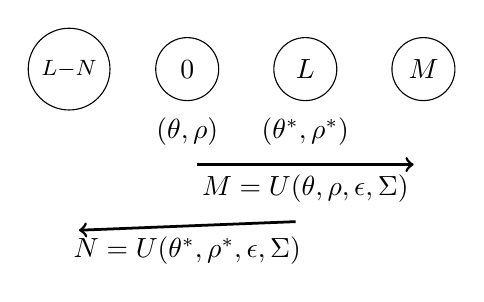
\begin{tikzpicture}[node distance=1.5cm and 0.75cm]
    % Top row nodes
    \node[circle,draw,minimum size=0.8cm] (LM) {\footnotesize $L{-}N$};
    \node[circle,draw,minimum size=0.8cm,right of=LM] (0) {$0$};
    \node[circle,draw,minimum size=0.8cm,right of=0] (L) {$L$};
    \node[circle,draw,minimum size=0.8cm,right of=L] (N) {$M$};
    
    % 2nd row nodes
    \node[below = 0.05cm of LM] (n_a1) {$\strut$};
    \node[below = 0.05cm of 0] (theta_rho) {$\strut (\theta, \rho)$};
    \node[below = 0.05cm of L] (theta_rho_star) {$\strut (\theta^*, \rho^*)$};
    \node[below = 0.05cm of N] (n_a2) {$\strut$};

    
    % 3rd row arrow
    \node[below = -0.25cm of n_a1] (n_a3) {$\strut$};
    \node[below = -0.25cm of theta_rho] (start_arrow2) {$\strut$};
    \node[below = -0.25cm of theta_rho_star] (n_a4) {$\strut$};
    \node[below = -0.25cm  of n_a2] (end_arrow2) {$\strut$};
    \draw[->, line width=1pt] (start_arrow2) -- (end_arrow2) node[midway, below] {$M = U(\theta, \rho, \epsilon, \Sigma)$};
    
    % 4th row arrow
    \node[below = 0.05cm of n_a4] (start_arrow1) {$\strut$};
    \node[below = 0.05cm of n_a3] (end_arrow1) {$\strut$};
    \draw[->, line width=1pt] (start_arrow1) -- (end_arrow1) node[midway, below] {$N = U(\theta^*, \rho^*, \epsilon, \Sigma)$};
\end{tikzpicture}
    \caption{\it {\bfseries U-turn evaluations for adaptive sampler.} The top row shows number of leapfrog steps in circles.  The second row shows positions and momenta for two states in phase space.  The third row shows the first evaluation of $U()$, which is forward in time $M$ steps from 0.  The number of steps $L$ for the proposal is chosen randomly, producing the proposal $(\theta^*, \rho^*)$.  The fourth row shows the second evaluation of $U()$ backwards in time from $L$ for $N$ steps.  If $L - N > 0,$ the proposal is rejected.}
    \label{fig:adaptive-u-turns}
\end{figure}

The leapfrog steps carried out by this algorithm are shown in .  

Figure~\ref{fig:adaptive-u-turns} shows a single step of the algorithm.  The basic idea is to uniformly sample of number of steps up to the number of steps possible before a U-turn, which determines the conditional distribution of number of steps.  To preserve detailed balance, the trajectory from the selected point backward in time is evaluated until it makes a U-turn and the probability of selecting the initial state (i.e., the same number of steps) is used to balance the selection.  

To make this algorithm more precise, let $U^{\textrm{dist}}(\theta, \rho, \epsilon, \Sigma)$ be defined to be the maximum number of leapfrog steps that can be taken from position $\theta$ with momentum $\rho$, using step size $\epsilon$ and metric $\Sigma,$ before the next step brings you closer to where you started,
\begin{equation}
\textrm{UTurn}(\pos{\theta}{0}, \pos{\rho}{0}, \epsilon, \Sigma)
= \textrm{arg min}_{N \in \mathbb{N}} \ \left(\pos{\theta}{N} - \pos{\theta}{0}\right) \cdot \pos{\rho}{N} < 0,
\end{equation}
where $\left(\pos{\theta}{n}, \pos{\rho}{n}\right)$ is the position in phase space after $n$ leapfrog steps from $\left(\pos{\theta}{0}, \pos{\rho}{0}\right)$ with step size $\epsilon$ and metric $\Sigma.$  This the definition of $\textrm{UTurn}$ in hand, the conditional distribution of step sizes can be defined as
\begin{equation}
p(L \mid \theta, \rho, \epsilon, \Sigma)
= \textrm{uniform}(L \mid 1, \textrm{UTurn}(\theta, \rho, \epsilon, \Sigma).
\end{equation}

One of the tricks NUTS uses to take such long jumps is to bias the selection of a candidate toward the end of the Hamiltonian trajectory \cite{HoGe2014}.  To create a simple approximation to this, the uniform distribution can be restricted to the latter part of the trajectory by changing the lower bound from 1 to something greater.  Any number between 0 and $M = \textrm{Uturn}(\theta, \rho, \epsilon, \Sigma)$ is valid as a lower bound, and we will evaluate the choices 1, $\lfloor \frac{1}{2} \cdot M \rfloor$, and $\lfloor \frac{3}{4} \cdot M \rfloor$.  Each subsequent choice increases the trajectory length of accepted proposals, but also lowers the probability of acceptance due to the reversibility condition.

\section{Non-uniform conditional distributions} \label{sec:nonuniform}

Non-uniform distributions may also be used.  For example, a binomial distribution for the number of steps could be defined for a fixed $\phi \in (0, 1)$ as 
\begin{equation}
    p(L \mid \theta, \rho, \epsilon, \Sigma)
    = \textrm{binomial}\!\left(L \mid \phi, \textrm{UTurn}(\theta, \rho, \epsilon, \Sigma)\right).
\end{equation}
The expected value of $L$ starting from $(\theta, \rho)$ is thus $\phi \cdot \textrm{UTurn}(\theta, \rho, \epsilon, \Sigma).$


\section{Detailed comparison to NUTS}

\begin{funding}
N.~Bou-Rabee has been partially supported by NSF Grant No.~DMS-2111224.
\end{funding}

\printbibliography

\appendix
{ \color{magenta}

IN PROGRESS: Nawaf: don't review this yet, i couldnt  finish it because Bob and I needed to work out some stuff with the simulations

\section{Proof of correctness}

The correctness of the algorithm in Figure ~\ref{fig:general-self-tuning-step} reduces to the following general lemma. Briefly, this lemma justifies applying the Metropolis-Hastings accept/reject step to a deterministic proposal given by a measure preserving involution. 

This will provide the proof of correctness as a consequence. Indeed, the algorithm in Figure ~\ref{fig:general-self-tuning-step} is nothing but Gibbs-like resampling of the velocity $\rho$ and tuning variable $\alpha$ interleaved with Metropolis-Hastings applied to the proposal $S \circ F(\alpha)$. 

\begin{lemma} \label{lem:DeterministicMetropolization}    
Suppose that $(\mathbb{S}, \mathcal{F}, \lambda)$ is a measure space, $\pi$ is a probability measure with density $ \gamma$ with respect to $\lambda$, and $F: \mathbb{S}\to \mathbb{S}$ is a measurable involution which preserves $\lambda$. Given a state $G \in \mathbb{S}$, define a Markov transition kernel by the following procedure:
\begin{itemize}
    \item Draw $\mathcal{U} \sim \operatorname{Unif}([0,1])$.
    \item Set $G' = F(G)$ if  $\mathcal{U} \le \min\left(1, \frac{\gamma(F(G'))}{\gamma(F(G))} \right)$ and $G' = G$ otherwise.
\end{itemize}
Then, this transition is reversible with respect to $\pi$.
\end{lemma}


\begin{proof}
It suffices to show that \[
\prb(G  \in A , G' \in B) =  \prb(G'  \in A , G \in B) \;, 
\] 
for all measurable sets $A,B$.
Let $\beta(x,F(x)) = \min \left(1, \frac{\gamma(F(x))}{\gamma(x)} \right)$. The above procedure gives the transition kernel $p(x, A) = \beta(x,F(x)) \delta_{F(x)}(A) + (1 - \beta(x, F(x))) \delta_{x}$. Hence,
\begin{align}
\prb(G & \in A , G' \in B) = \int_A p(x,B) \pi(dx) \notag \\
&= \int_A \beta(x, F(x)) I_B(F(x)) + (1 - \alpha(x,F(x))) I_B(x) \pi(dx) \label{eq:metrodef} \\
&= \int_\mathbb{S} \beta(x, F(x)) I_B(F(x)) I_A(x) + (1 - \alpha(x,F(x)))I_A(x)I_B(x) \pi(dx) \label{eq:metropolisexpansion}
\end{align}

The second term in the integral is already symmetric in the sets $A,B$ - so we turn out attention to the first. For this term, we use the identity $a \min(1, \frac{b}{a}) = b \min(1, \frac{a}{b})$ valid for all $a, b \ne 0$. 

\begin{align}
\int_\mathbb{S} \beta(x, F(x))& I_B(F(x)) I_A(x) \pi(dx) = \int_\mathbb{S} \beta(x, F(x)) I_B(F(x)) I_A(x) \gamma(x) \lambda(dx) \notag \\
&= \int_\mathbb{S} I_B(F(x)) I_A(x) \gamma(x) \min \left(1, \frac{\gamma(F(x))}{\gamma(x)} \right) \lambda (dx) \notag \\
&= \int_X I_B(F(x)) I_A(x) \gamma(F(x)) \min \left(1, \frac{\gamma(x)}{\gamma(F(x))} \right) \lambda (dx) \notag 
\end{align}
But, since $F$ preserves $\lambda$ and is an involution we have - in turn- 
\begin{multline}
\int_\mathbb{S} I_B(F(x)) I_A(x) \gamma(F(x)) \min \left(1, \frac{\gamma(x)}{\gamma(F(x))} \right) \lambda (dx) = \\
\int_\mathbb{S} I_B(F(F(x))) I_A(F(x)) \gamma(F(F(x))) \min \left(1, \frac{\gamma(F(x))}{\gamma(F(F(x)))} \right) \lambda (dx) \\
=\int_X I_B(x) I_A(F(x)) \gamma(x) \min \left(1, \frac{\gamma(F(x))}{\gamma(x))} \right) \lambda (dx) \\
=\int_X \beta(x, F(x)) I_B(x) I_A(F(x)) \gamma(x) \pi (dx) \\
\label{eq:metroaftercov}
\end{multline}

Inserting (\ref{eq:metroaftercov}) into (\ref{eq:metropolisexpansion}) and comparing with (\ref{eq:metrodef}) we observe 
\[\prb(G \in A , G' \in B) = \prb(G \in B , G' \in A)\]
as required.
\end{proof}

With this lemma in hand we now prove the correctness of the algorithm

\begin{theorem}
The iterates $(\theta_0, \rho_0), (\theta_1, \rho_1), \dots $ of the algorithm described in Figure ~\ref{fig:general-self-tuning-step} define a Markov Chain with stationary measure $\mu(d \theta \, d \rho) = \frac{1}{Z} e^{-U(x) + \frac{1}{2} |\rho|^2} m(d \theta \, d \rho)$.
\end{theorem}

\begin{proof}
In the notation of Figure ~\ref{fig:general-self-tuning-step} suppose  $(\theta_0, \rho_0) \sim \mu$. Note that then, $(\theta_0, \rho_0, \alpha) \sim \mu_e$. 

Define a map $G(\theta, \rho, \alpha) = (S \circ F(\alpha)(\theta, \rho), \alpha)$. As $S \circ F(\alpha)$ is an involution $G$ is automatically an involution. Additionally $S \circ F(\alpha)$ preserves Lebesgue measure for every fixed $\alpha$ and hence by Fubini's theorem $G$ preserves $(m \otimes \eta)$ on $\mathbb{R}^{2d} \times \mathcal{A}$.

Let $\mathcal{U} \sim \operatorname{Unif}([0,1])$ and set 

\[
(\theta_1, \rho_1) =\begin{cases}
(\theta^*, \rho^*) \quad \text{if  } e^{-\Delta H(\theta_0, \rho_0)} \frac{p(\alpha \mid S \circ F(\alpha)(\theta_0, \rho_0)}{p(\alpha \mid \theta, \rho)} \leq \mathcal{U} \\
(\theta_0, \rho_0) \quad \text{else}
\end{cases}
\]

\[ \mathbb{P}((\theta_0, \rho_0) \in A, (\theta^*, \rho^*) \in B)  = \mathbb{P}(\theta^* \in A, \theta_0 \in B)\]

Drawing $\rho_0 \sim \operatorname{Normal}(0,I_{d \times d})$ and $\alpha \sim p(\cdot \mid \theta_0, \rho_0)$ gives $(\theta_0, \rho_0, \alpha) \sim \mu_e$. Note now that $\mu_e$ has density $\gamma =  $    
\end{proof}


\label{app:proof_of_correctness}
}
\end{document}



